\chapter{Elasticity in port-Hamiltonian form}

\epigraph{I try not to break the rules but merely to test their elasticity.}{\textit{Bill Veeck}}
\minitoc

\lettrine{\color{theme}{C}}ontinuum mechanics is the mathematical description of how materials behave kinematically under external excitations. In this framework, the microscopic structure of a material body is neglected and a macroscopic viewpoint, that describes the body as a continuum, is adopted. This leads to a PDE based model. In this chapter, the general linear elastodynamics problem is recalled. A suitable port-Hamiltonian formulation is then derived.

\section{Continuum mechanics}
In this section, the main concepts behind a deformable continuum are briefly recalled following \cite{lee2012mixed}. For a detailed discussion on this topic, the reader may consult \cite{abeyaratne2012notes,landau2012elasticity}. 

\subsection{Non linear formulation of elasticity}

The bounded region of $\mathbb{R}^d \; (d=2, 3)$ occupied by a solid is called configuration. The reference configuration $\Omega$ is the domain that a bodies occupies at the initial state. To describe how the body deforms in time the deformation map $\bm\Phi: \Omega \times [0, T_f] \rightarrow \Omega' \subset \mathbb{R}^d$ is introduced. This map is differentiable and orientation preserving and the image of $\Omega$ under $\bm\Phi(\cdot, t) \; \forall t \in [0, T_f]$ is called the deformed configuration $\Omega_t$. Given a specific point in the reference frame its image is denoted by $\bm{y} = \bm{\Phi}(\bm{x}, t)$. The gradient of the deformation map is called the deformation gradient $\bm{F}:=\nabla_x\bm{\Phi} = \diffp{\bm{y}}{\bm{x}}$. A rigid deformation maps a point $\bm{x} \in \Omega \rightarrow \bm{A}(t) \bm{x} + \bm{b}(t)$, where $\bm{A}(t)$ is an orthogonal matrix and $\bm{b}(t)$ an $\mathbb{R}^d$ vector. A differentiable deformation map $\bm\Phi$ is a rigid deformation iff $\bm{F}^\top \bm{F} - \bm{I} = 0$,  where $\bm{I}$ is the identity in $\mathbb{R}^{d\times d}$ (for the proof see \cite{ciarlet1988mathematical}, page 44). For this reason, a suitable measure of the deformation is the Green-St.Venant strain tensor $\frac{1}{2} (\bm{F}^\top \bm{F} - \bm{I})$.  \\
A quantity of interest is the displacement $\bm{u}: \Omega \times [0, T_f] \rightarrow \mathbb{R}^d$ with respect to the reference configuration. It is defined as $\bm{u}(\bm{x}, t) = \bm{\Phi}(\bm{x}, t) - \bm{x}$. The gradient of the displacement verifies $\nabla_x \bm{u} = \bm{F} - \bm{I}$. The strain tensor can now be written in terms of the displacement
\begin{equation*}
\begin{aligned}
\frac{1}{2} (\bm{F}^\top \bm{F} - \bm{I}) &= \frac{1}{2}\left[(\nabla_x \bm{u} + \bm{I})^\top (\nabla_x \bm{u} + \bm{I}) - \bm{I}\right] \\
&= \frac{1}{2}\left[\nabla_x \bm{u} + (\nabla_x \bm{u})^\top + (\nabla_x \bm{u})^\top (\nabla_x \bm{u})\right],
\end{aligned}
\end{equation*}
or in components 
\begin{equation*}
\frac{1}{2} ({F}_{ik}^\top {F}_{kj} - {I}_{ij}) = \frac{1}{2} \left(\diffp{u_i}{x_j} + \diffp{u_j}{x_i} + \diffp{u_i}{x_j}\diffp{u_j}{x_i}\right).
\end{equation*}

To state the balance laws the actual deformed configuration is considered. The linear and angular momentum in a subdomain $\omega_t \subset \Omega_t$ are computed as 
\begin{equation*}
\int_{\omega_t} \rho \, \bm{v} \d{\omega_t}, \qquad \int_{\omega_t} \rho \, \bm{y} \times \bm{v} \d{\omega},
\end{equation*}
where $\rho$ is the mass density and the velocity $\bm{v} = \frac{D\bm{u}}{Dt}(\bm{y},t) = \diffp{\bm{u}}{t} + (\nabla_x \bm{u}) \cdot \bm{v}$ is material time derivative of the displacement (see \cite[Chapter 1]{abeyaratne2012notes}).  Let $\omega_{t, 1},\, \omega_{t, 2}$ be two subregions in a deformed continuum $\Omega_t$ with contacting surface $S_{12}$. There is a force acting on this surface for a continuum that is called stress vector or traction. If $\bm{n}$ is the outward normal at $\bm{y}$ on $S_{12}$ with respect to $\omega_{t, 1}$, then the surface force that $\omega_{t, 1}$ exerts on $\omega_{t, 2}$ is denoted by $\bm{t}(\bm{y}, \bm{n}) \in \mathbb{R}^d$. By the Newton third law, the surface force that $\omega_{t, 2}$ applies on $\omega_{t, 1}$ is given by $\bm{t}(\bm{y}, -\bm{n}) = - \bm{t}(\bm{y}, \bm{n})$. It is assumed that the linear and angular momentum balance hold for any subregion $\omega_t \in \Omega_t$ 
\begin{align*}
	\diff{}{t} \int_{\omega_t} \rho \bm{v} \d{\omega_t} &= \int_{\partial \omega_t} \bm{t}(\bm{y}, \bm{n}) \d{S} + \int_{\omega_t} \bm{f} \d{\omega_t}, \\
	\diff{}{t} \int_{\omega_t} \rho\bm{y} \times \bm{v} \d{\omega_t} &= \int_{\partial \omega_t} \bm{y} \times \bm{t}(\bm{y}, \bm{n}) \d{S} + \int_{\omega_t} \bm{y} \times \bm{f} \d{\omega_t}, \\
\end{align*}
where $\partial \omega_t$ stands for the boundary surface of the subdomain $\omega_t$, $\bm{n}$ is the outward normal to the surface $\partial\omega_t$ and $\bm{f}$ represents an exterior body force. The following theorem characterizes the stress vector (see \cite[Chapter 2]{ciarlet1988mathematical}):

\begin{theorem}[Cauchy’s theorem]
If the linear and angular momenta balance hold, then there exists a matrix-valued function $\bm{\Sigma}$ from $\Omega_t$ to $\mathbb{S}$ such
that $\bm{t}(\bm{y}, \bm{n}) = \bm{\Sigma}(\bm{y}) \bm{n}, \; \forall \bm{y} \in \Omega_t$ where the right-hand side is the matrix-vector multiplication.
\end{theorem}
The set $\mathbb{S}=\mathbb{R}^{d\times d}_{\mathrm{sym}}$ denotes the field of symmetric matrices in $\mathbb{R}^{d\times d}$. The symmetry of the stress tensor $\bm{\Sigma}$ is due to the balance of angular momentum. The divergence theorem can then be applied
\begin{equation*}
\int_{\partial \omega_t} \bm{\Sigma} \, \bm{n} \d{S} = \int_{\omega_t} \nabla_y \cdot\bm{\Sigma} \d{\omega},
\end{equation*}
where $\nabla_y \cdot$ is the tensor divergence with respect to the deformed configuration, $\nabla_y \cdot\bm{\Sigma} = \sum_{i=1}^{d}\diffp{\Sigma_{ij}}{y_i}$.
Because the considered subregion $\omega_t$ is arbitrary, using the linear balance momentum and the conservation of mass the following PDE is found
\begin{equation*}
	\rho \frac{D\bm{v}}{Dt} - \nabla_y \cdot{\bm{\Sigma}} = \bm{f}, \qquad \bm{y} \in \Omega_t.
\end{equation*}
This equation is written with respect to the deformed configuration $\Omega_t$. For a detailed derivation of this equation the reader may consult \cite[Chapter 4]{abeyaratne2012notes}. To obtain a closed formulation, the constitutive law, namely the link between $\bm{\Sigma}$ and the strain tensor $\frac{1}{2} (\bm{F}^\top \bm{F} - \bm{I})$, has to be introduced. In the next such relation will be investigated for the case of linear elasticity.

\subsection{The linear elastodynamics problem}\label{sec:linElas}
Whenever deformations are small, $\norm{\nabla_x\bm{u}} \ll 1$, then the reference and deformed configurations are almost indistinguishable $\bm{y} = \bm{x} + \bm{u} = \bm{x}  + O(\nabla_x\bm{u}) \approx \bm{x}$. This allows to write the linear momentum balance in the reference configuration
\begin{equation*}
	\rho \diffp{\bm{v}}{t}(\bm{x, t}) - \Div(\bm\Sigma(\bm{x}, t)) = \bm{f}, \qquad \bm{x} \in \Omega.
\end{equation*}
The material derivative simplifies to a partial one. The operator $\Div$ is the divergence of a tensor field with respect to the reference configuration
\begin{equation*}
\Div(\bm\Sigma(\bm{x}, t)) = \nabla_x \cdot \bm\Sigma(\bm{x}, t) = \left(\sum_{i=1}^{d}\diffp{\Sigma_{ij}}{x_i}\right)_{1 \leq j \leq d}.
\end{equation*}
Furthermore, the non-linear terms in the Green-St. Venant strain tensor can be dropped
\begin{equation*}
\frac{1}{2} (\bm{F}^\top \bm{F} - \bm{I}) = \frac{1}{2}\left[\nabla_x \bm{u} + (\nabla_x \bm{u})^\top + (\nabla_x \bm{u})^\top (\nabla_x \bm{u})\right]
\approx \frac{1}{2}\left[\nabla_x \bm{u} + (\nabla_x \bm{u})^\top\right].
\end{equation*}
The linearized strain tensor (also called infinitesimal strain tensor) is the symmetric gradient of the displacement
\begin{equation}
\bm{\varepsilon} := \Grad\bm{u}, \where \Grad\bm{u} = \frac{1}{2}\left[\nabla_x \bm{u} + (\nabla_x \bm{u})^\top\right].
\end{equation}

To obtain a closed system of equations, it is now necessary to characterize the relation between stress and strain. This relation is normally called \textit{constitutive law}. In the following, the particular case of elastic materials is considered. These are able to resist distorting excitations and return to its original size and shape when these are removed. For this class of materials, the stress tensor is solely determined by the deformed configuration at a given time (Hooke's law)
\begin{equation*}
\bm{\Sigma}(\bm{x}) = \bm{\mathcal{D}}(\bm{x}) \, \bm{\varepsilon}(\bm{u}(\bm{x})).
\end{equation*}
The \textit{stiffness tensor} or \textit{elasticity tensor} $\bm{\mathcal{D}} : \mathbb{S} \rightarrow \mathbb{S}$ is a rank 4 tensor that is symmetric positive definite and uniformly bounded above and below. Because of symmetry, its components satisfy
\begin{equation*}
\mathcal{D}_{ijkl} = \mathcal{D}_{jikl} = \mathcal{D}_{klij}.
\end{equation*}
From the uniform boundedness of $\bm{\mathcal{D}}$, the map
$\bm{\mathcal{D}}: L^2 (\Omega; \mathbb{S}) \rightarrow L^2 (\Omega; \mathbb{S})$ is a symmetric positive definite bounded linear operator ($L^2 (\Omega; \mathbb{S})$ is the space of square integrable symmetric tensor-valued functions). The compliance tensor $\bm{\mathcal{C}}$ is defined by $\bm{\mathcal{C}} = \bm{\mathcal{D}}^{-1}$ . Thus $\bm{\mathcal{C}} : \mathbb{S} \rightarrow \mathbb{S}$ is as well symmetric positive definite and uniformly bounded above and below. An isotropic
elastic medium has the same kinematic properties in any direction and at each point. If an elastic medium is isotropic, then the stiffness and compliance tensors assume the form
\begin{equation}
\bm{\mathcal{D}}(\cdot) = 2\mu (\cdot) + \lambda \Tr(\cdot)\bm{I}, \qquad \bm{\mathcal{C}}(\cdot) = \frac{1}{2\mu}\left[(\cdot) - \frac{\lambda}{2\mu + d\lambda}\Tr(\cdot)\bm{I}\right], \qquad d= \{2,3\},
\end{equation}
where  $\Tr$ is the trace operator and the positive scalar functions $\mu, \lambda$, defined on $\Omega$, are called the Lam\'e coefficients. In engineering applications it is easier to compute experimentally two other parameters: the Young modulus $E$ and  Poisson's ratio $\nu$. Those are expressed in terms of the Lam\'e  coefficients as 
\begin{equation}
\nu =\frac{\lambda}{2(\lambda +\mu)}, \qquad 
E=\frac{\mu (3\lambda +2\mu)}{\lambda +\mu},
\end{equation}
and conversely
\begin{equation}
\lambda =\frac {E \nu }{(1+\nu )(1-2\nu )}, \qquad
\mu = \frac{E}{2(1+\nu)}.
\end{equation}
The stiffness and compliant tensor assume the expressions
\begin{align}
	\bm{\mathcal{D}}(\cdot) &= \frac{E}{1+\nu} \left[(\cdot) + \frac{\nu}{1-2\nu}\Tr(\cdot)\bm{I}\right], \label{eq:stiff3D} \vspace{3pt}\\
	\bm{\mathcal{C}}(\cdot) &= \frac{1+\nu}{E}\left[(\cdot) - \frac{\nu}{1+\nu(d-2)}\Tr(\cdot)\bm{I}\right].
\end{align}
The linear elastodynamics problem is formulated through a vector-valued PDE
\begin{equation}\label{eq:lin_elastodyn}
\rho \diffp[2]{\bm{u}}{t} - \Div(\bm{\mathcal{D}} \Grad \bm{u}) = \bm{f}.
\end{equation}  
The classical elastodynamics problem is expressed in terms of the displacement as the unknown. This PDE goes together with appropriate boundary conditions that will be specified in \ref{sec:pHelas}.

\section{Port-Hamiltonian systems}

Before introducing the pH formulation of the elastodynamics problem, the main concept behind this formalism are recalled. First, the concept of Stokes-Dirac structure is presented. This is normally introduced by making use of a differential geometry approach. The interested reader may consult \cite[Chapter 2]{kotyczka2019numerical}. Despite being really insightful in terms of geometrical structure, this approach does not encompass the case of higher-order differential operators. An extension in this sense is still an open question. Since bending problems in elasticity introduce higher-order differential operators, the language of PDE will be privileged over the one of differential forms. To have the most suitable definition of Stokes-Dirac structure for flexible systems, the approach adopted in \cite{macchelli2005modelling} is here recovered. \\

Second, distributed port-Hamiltonian systems are introduced, in connection with the underlying Stokes-Dirac structure. PHs as boundary control systems have been analyzed deeply in one geometrical dimension \cite{zwart2012,legorrec2005}. Here, a more general definition is given. The complete characterization of pH in arbitrary dimension is still an open research field. Two notable exceptions (\cite{zwart2015wave,skrepek2019wellposedness}) provide partial answers to this problem. The first demonstrate the well-posedness of the linear wave equation in arbitrary geometrical dimensions. The second generalizes this result to treat the case of generic first order linear pHs in arbitrary geometrical dimensions.

 
\subsection{The Stokes-Dirac structure}

In the section the concept of Stokes-Dirac structure for distributed, i.e. infinite-dimensional, pHs is introduced. First, the finite-dimensional case is considered. Then, to introduce the infinite-dimensional extension of Dirac structure, namely the Stokes-Dirac structure, the differential operators that come into play are characterized. 

\subsubsection{Dirac Structures}
Consider a  finite dimensional space ${F}$ over the field $\mathbb{R}$ and ${E} \equiv {F}'$ its dual, i.e. the space of linear operator $\mathbf{e} : {F} \rightarrow \mathbb{R}$. The elements of $\mathit{F}$ are called flows, while the elements of ${E}$ are called efforts. Those are port variables and their combination gives the power flowing inside the system. The space ${B} = {F} \times {E}$ is called the bond space of power variables. Therefore the power is defined as  $\left\langle \mathbf{e}, \mathbf{f} \right\rangle = \bm{e}(\mathbf{f})$, where $\left\langle \mathbf{e} , \mathbf{f} \right\rangle$ is the dual product between $\mathbf{f}$ and $\mathbf{e}$.
\begin{definition}[\cite{courant1990}, Def. 1.1.1]
	Given the finite-dimensional space ${F}$ and its dual ${E}$ with respect to the inner product $\left\langle \cdot , \cdot \right\rangle : {F} \times {E} \rightarrow \mathbb{R}$, define the symmetric bilinear form:
	\begin{equation}
	\bilprod{(\mathbf{f}_1, \mathbf{e}_1)}{(\mathbf{f}_2, \mathbf{e}_2)} := \inner{\mathbf{e}_1}{\mathbf{f}_2} +  \inner{\mathbf{e}_2}{\mathbf{f}_1}, \where (\mathbf{f}_i, \mathbf{e}_i) \in {B}, \; i = 1, 2
	\end{equation}
	
	A Dirac structure on ${B} := {F} \times {E}$ is a subspace ${D} \subset {B}$, which is maximally isotropic under $\left\langle \left\langle \cdot, \cdot \right\rangle \right\rangle$.	Equivalently, a Dirac structure on ${B} := {F} \times {E}$ is a subspace ${D} \subset {B}$ 	which equals its orthogonal complement with respect to $\left\langle \left\langle \cdot, \cdot \right\rangle \right\rangle: {D} ={D}^\perp$.
\end{definition}
This definition can be extended to consider distributed forces and dissipation \cite{villegas2007}.
\begin{proposition}
	\label{prop:Dirac}
	Consider the space of power variables ${F} \times {E}$ and let ${X}$ denote an $n$-dimensional space, the space of energy variables. Suppose that ${F} := ({F}_s, \ {F}_e )$ and that ${E} := ({E}_s,  \ {E}_e )$, with $\text{dim} \, {F}_s = \text{dim} \, {E}_s = n$ and $\text{dim} \, {F}_e = \text{dim} \, {E}_e = m$. Moreover, let $\mathbf{J}(\mathbf{x})$ denote
	a skew-symmetric matrix of dimension $n$ and $\mathbf{B}(\mathbf{x})$ a matrix of dimension $n \times m$. Then, the set
	\begin{equation}
	{D} := \left\{ (\mathbf{f}_s, \mathbf{f}_e , \mathbf{e}_s ,\mathbf{e}_e ) \in {F} \times {E} \vert \quad \mathbf{f}_s = - \mathbf{J}(\mathbf{x}) \mathbf{e}_s - \mathbf{B}(\mathbf{x}) \mathbf{f}_e, \; \mathbf{e}_e = \mathbf{B}(\mathbf{x})^\top \mathbf{e}_s \right\}
	\end{equation}
	is a Dirac structure.
\end{proposition}

\subsubsection{Finite-dimensional port-Hamiltonian systems}
Consider the time-invariant dynamical system:
\begin{equation}
\label{eq:finitePH}
\begin{cases}
\dot{ \mathbf{x} } &= \mathbf{J}(\mathbf{x}) \nabla H(\mathbf{x}) + \mathbf{B}(\mathbf{x})\mathbf{u}, \\
\mathbf{y} &= \mathbf{B}(\mathbf{x})^\top \nabla H(\mathbf{x}),
\end{cases}
\end{equation}
where $ H(\mathbf{x}) : X \rightarrow \mathbb{R} $, the Hamiltonian, is a real-valued function bounded from below. Such a system is called port-Hamiltonian, as it arises from the Hamiltonian modelling of a physical system and it interacts with the environment through the input $\mathbf{u}$, included in the formulation. The connection with the concept of Dirac structure is achieved by considering the following port behavior:
\begin{equation}
\begin{aligned}
\mathbf{f}_s &= - \dot{\mathbf{x}}, \qquad 
&\mathbf{e}_s &= \nabla{H}(\mathbf{x}), \\
\mathbf{f}_e &= \mathbf{u}, \qquad
&\mathbf{e}_e &= \mathbf{y}. \\
\end{aligned}
\end{equation}
With this choice of the port variables system \eqref{eq:finitePH} defines, by Proposition \ref{prop:Dirac}, a Dirac structure. Dissipation and distributed forces can be included and the corresponding system defines an extended Dirac structure, once the proper port variables have been introduced.

\subsubsection{Constant matrix differential operators}

Let $\Omega$ denote a compact subset of $\mathbb{R}^d$ representing the spatial domain of the distributed parameter system. Then, let ${U} = C^{\infty}(\Omega, \mathbb{R}^{q_u})$ and ${V}= C^{\infty}(\Omega, \mathbb{R}^{q_v})$ denote the sets of smooth functions from $\Omega$ to $\mathbb{R}^{q_u}$ and $\mathbb{R}^{q_v}$ respectively.
\begin{definition}
	A constant matrix differential operator of order $n$ is a map $\mathcal{L}:{U} \rightarrow {V}$ such that, given $\bm{u} = (u_1 , \dots , u_{q_u}) \in {U}$ and $\bm{v} = (v_1 , . . . , v_{q_v}) \in {V}$:
	\begin{equation}
	\label{eq:diffOp}
	\bm{v} = \mathcal{L} \bm{u} \iff \bm{v} := \sum_{|\alpha|=0}^n  \bm{P}_{\alpha} \partial^{\alpha} \bm{u},
	\end{equation}
	where $\alpha := (\alpha_1, \dots , \alpha_d)$ is a multi-index of order $|\alpha| := \sum_{i=1}^d \alpha_i$, $\bm{P}_\alpha$ is a set of constant real $q_v \times q_u$ matrices and $\partial^{\alpha} := \partial_{x_1}^{\alpha_1} \dots \partial_{x_d}^{\alpha_d}$ is a differential operator of order $|\alpha|$ resulting from a combination of spatial derivatives. 
\end{definition}
The following definition, instrumental for the case of dpHs, is a simplified version of \eqref{def:foradj}.
\begin{definition}
	Consider the constant matrix differential operator \eqref{eq:diffOp}. Its formal adjoint is the map $\mathcal{L}^*$ from ${V}$ to ${U}$ such that:
	\begin{equation}
	\bm{u} = \mathcal{L}^* \bm{v} \iff \bm{u} := \sum_{|\alpha|=0}^n  (-1)^{|\alpha|} \bm{P}_{\alpha}^\top \partial^{\alpha} \bm{v}.
	\end{equation}
\end{definition}

\begin{remark}[Differences between adjoint and formal adjoint]
The definition of formal adjoint is such that the integration by parts formula is respected
\begin{equation*}
\int_{\Omega} \bm{a} \cdot (\mathcal{L}\bm{b}) \d\Omega = \int_{\Omega} (\mathcal{L}^*\bm{a}) \cdot \bm{b} \d\Omega,
\end{equation*}
where $\bm{a} \in C^{\infty}_0(\Omega, \mathbb{R}^{q_u}), \; \bm{b} \in C^{\infty}_0(\Omega, \mathbb{R}^{q_v})$ are smooth functions with compact support. This corresponds to the adjoint definition for an operator between $L^2$ spaces of square integrable functions
\begin{equation*}
\inner[L^2(\Omega, \mathbb{R}^{q_v})]{\bm{a}}{\mathcal{L}\bm{b}} = \inner[L^2(\Omega, \mathbb{R}^{q_u})]{\mathcal{L}^*\bm{a}}{\bm{b}}.
\end{equation*}
That means that, contrarily to the adjoint of an operator, the formal adjoint definition does not regard the actual domain of the operator nor the boundary conditions. For example, the differential operators $\div,\, \grad$ are unbounded in the ${L}^2$ topology. Whenever unbounded operators are considered, it is important to define their domain. To avoid the need of specifying domains, the notion of formal adjoint can be evoked. The formal adjoint respects the integration by parts formula and is defined only for sufficiently smooth functions with compact support. In this sense $\div, \grad$ are formally skew-adjoint, since for smooth functions with compact support, it holds
\begin{equation*}
\left\langle \bm{y}, \, \grad({x}) \right\rangle_{{L}^2(\Omega, \mathbb{R}^{3})} 
\underbrace{=}_{\text{I.B.P.}} -\left\langle\div(\bm{y}), \, {x} \right\rangle_{{L}^2(\Omega, \mathbb{R})},
\end{equation*}
for $\bm{Y} \in C_0^\infty(\Omega, \mathbb{R}^{n}), \; {x} \in C_0^\infty(\Omega)$ (I.B.P. stands for integration by parts). The definition of the domain of the operators, that requires the knowledge of the boundary conditions, has not been specified. 
\end{remark}

\begin{definition}
	\label{def:skewOp}
	Let $W = C^{\infty}(\Omega, \mathbb{R}^{q})$ be the space of vector-valued smooth functions and $\mathcal{J}: W \rightarrow W$ a constant matrix differential operator. Then, $\mathcal{J}$ is formally skew-adjoint (or skew-symmetric) if and only if $\mathcal{J} = -\mathcal{J}^*$. This corresponds to the algebraic condition
	\begin{equation}
	\bm{P}_{\alpha} = (-1)^{|\alpha| + 1} \bm{P}_{\alpha}^\top, \quad \forall \alpha.
	\end{equation}
\end{definition}
An important relation between a differential operator and its adjoint is expressed by the following theorem.
\begin{theorem}[\cite{rogers2004pde}, Chapter 9, theorem 9.37]
	Consider a matrix differential operator $\mathcal{L}$ and let $\mathcal{L}^*$ denote its formal adjoint. Then, for each function $\bm{u} \in {U}$ and $\bm{v} \in {V}$:
	\begin{equation}
	\int_{\Omega} \left( \bm{v}^\top \mathcal{L} \bm{u} - \bm{u}^\top \mathcal{L}^* \bm{v}\right) \d\Omega= \int_{\partial \Omega} \widetilde{\mathcal{B}}_{\mathcal{L}}(\bm{u}, \bm{v}) \d{A},
	\end{equation}
	where $\widetilde{\mathcal{B}}_{\mathcal{L}}$ is a differential operator induced on the boundary $\partial\Omega$ by $\mathcal{L}$, or equivalently:
	\begin{equation}
	\bm{v}^\top \mathcal{L} \bm{u} - \bm{u}^\top \mathcal{L}^* \bm{v} = \mathrm{div} \, \widetilde{\mathcal{B}}_{\mathcal{L}}(\bm{u}, \bm{v}).
	\end{equation}
\end{theorem}
It is important to note that $\widetilde{\mathcal{B}}_{\mathcal{L}}$ is a constant differential operator. The quantity $\widetilde{\mathcal{B}}_{\mathcal{L}}(\bm{u}, \bm{v})$ is a constant linear combination of the functions $\bm{u}$ and $\bm{v}$ together with their spatial derivatives up to a certain order and depending on $\mathcal{L}$.
\begin{corollary}
	Consider a skew-symmetric differential operator $\mathcal{J}$. Then, for each function $\bm{u} \in {U}$ and $\bm{v} \in {V}$ with $q_u = q_v = q$:
	\begin{equation}
	\int_{\Omega} \left( \bm{v}^\top \mathcal{J} \bm{u} + \bm{u}^\top \mathcal{J} \bm{v}\right) \d\Omega= \int_{\partial \Omega} \widetilde{\mathcal{B}}_{\mathcal{J}}(\bm{u}, \bm{v}) \d{A},
	\end{equation}
	where $\widetilde{\mathcal{B}}_{\mathcal{J}}$ is a symmetric differential operator on $\partial\Omega$ depending on the differential operator~$\mathcal{J}$.
\end{corollary}

\subsubsection{Constant Stokes-Dirac structures}
Following \cite{macchelli2005modelling}, let ${F}$ denote the space of flows, i.e. the space of smooth functions from the compact set $\Omega \subset \mathbb{R}^d$ to $\mathbb{R}^q$. For simplicity assume that  the space of efforts is ${E} \equiv {F}$ (generally speaking these spaces are Hilbert spaces linked by duality, as in \cite{villegas2007}). Given $\bm{f} = (f_1, \dots, f_q) \in {F}$ and $\bm{e} = (e_1, \dots, e_q) \in {E}$. Let $\bm{z} = \mathcal{B}_\partial(\bm{e})$ denote the boundary terms, where $\mathcal{B}_\partial$ provides the restriction on $\partial\Omega$ of the effort variables $\bm{e}$ and of their spatial derivatives of proper order. The associated boundary space is ${Z} := \left\{ \bm{z} \vert \; \bm{z} = \mathcal{B}_{\partial}(\bm{e})  \right\}$. Then, it holds
\begin{equation}
\int_{\partial \Omega} \widetilde{\mathcal{B}}_{\mathcal{J}}(\bm{e}_1, \bm{e}_2) \d{S} = \int_{\partial \Omega} \mathcal{B}_{\mathcal{J}}(\bm{z}_1, \bm{z}_2) \d{S}, \quad \text{with} \quad  \widetilde{\mathcal{B}}_\mathcal{J}(\cdot, \cdot) = \mathcal{B}_{\mathcal{J}}(\mathcal{B}_{\partial}(\cdot), \, \mathcal{B}_{\partial}(\cdot)).
\end{equation}
The following theorem characterizes Stokes-Dirac structures for pHs of arbitrary geometrical dimension and differential order.
\begin{proposition}[Proposition 3.3 \cite{macchelli2005modelling}]
	\label{prop:StokesDirac}
	
	Consider the space of power variables ${B} = {F} \times {E} \times {Z}$. The linear subspace ${D} \subset {B}$
	\begin{equation}
	{D}_{\mathcal{J}} = \left\{ (\bm{f}, \bm{e}, \bm{z}) \in  {F} \times {E} \times {Z} \; \vert \; \bm{f} = -\mathcal{J} \bm{e}, \; \bm{z} = \mathcal{B}_\partial(\bm{e}) \right\},
	\end{equation}
	is a Stokes–Dirac structure on $\mathcal{B}$ with respect to the pairing
	\begin{equation}
	\bilprod{(\bm{f}^1, \bm{e}^1, \bm{z}^1)}{(\bm{f}^2, \bm{e}^2, \bm{z}^2)}  := \int_{\Omega} \left( \bm{e}^{1 \top} \bm{f}^ 2 + \bm{e}^{2 \top} \bm{f}^1 \right) \d\Omega + \int_{\partial \Omega} \mathcal{B}_{\mathcal{J}}(\bm{z}^1, \bm{z}^2) \d{S}.
	\end{equation}
\end{proposition}
From this proposition, if $(\bm{f}, \bm{e}, \bm{z}) \in  D_{\mathcal{J}}$, then $\bilprod{(\bm{f}, \bm{e}, \bm{z})}{(\bm{f}, \bm{e}, \bm{z})}=0$, that is
\begin{equation}\label{eq:enbalstr}
\int_{\Omega} \bm{e}^\top \bm{f}  \d\Omega + \frac{1}{2} \int_{\partial \Omega} \mathcal{B}_{\mathcal{J}}(\bm{z}, \bm{z}) \d{S} = 0.
\end{equation}


This  relation expresses the  power  conservation property of the Stokes–Dirac structure. It states the relation between the variation of internal energy (the integral on the domain $\Omega$) with the power flowing through the boundary (the integral over $\partial\Omega$). Thanks to the power conservation property dpHs always dispose of an associated Stokes Dirac structure. This concept can be extended to consider dissipation or distributed forces. To this aim, it is necessary to include additional ports to account for the power exchange due to these effects (see Theorem 3.4 \cite{macchelli2005modelling}). 


\begin{remark}
	The constant Stokes-Dirac structure has been defined in case of smooth vector-valued functions for simplicity.  The definition is indeed more general and encompasses the case of more complex functional spaces, in particular the $L^2$ space of square integrable functions.  Linear elasticity for example is defined on a mixed function space of vector- and tensor-valued functions. The constant differential operator may contain intrinsic operators ($\mathrm{Div}, \, \mathrm{Grad}$) as it will be shown in \secref{sec:pHelas}. The result presented here remains valid provided that the proper {pairing is being chosen}. 
\end{remark}


\subsection{Distributed port-Hamiltonian systems}

A distributed conservative port-Hamiltonian system is defined by a set of variables that describes the unknowns, by a formally skew-adjoint differential operator, an energy functional and a set of boundary inputs and corresponding conjugated outputs. Such a system is described by the following set of equations
\begin{equation}\label{eq:phsys}
\begin{aligned}
\diffp{\bm{\alpha}}{t} &= \mathcal{J}\displaystyle \bm{e}, \vspace{3pt}\\
\bm{u}_\partial &= \mathcal{B}  \displaystyle \bm{e}, \vspace{3pt}\\
\bm{y}_\partial &= \mathcal{C} \displaystyle \bm{e}, \vspace{3pt}\\
\bm{e} &:= \displaystyle \diffd{H}{\bm{\alpha}}.
\end{aligned}
\end{equation}
The unknowns $\bm{\alpha}$ are called energy variables in the port-Hamiltonian framework, the formally skew-adjoint operator $\mathcal{J}$ is named interconnection operator (see appendix \ref{app:math}, Def. \ref{def:foradj} for a precise definition of formal skew adjointness). $\mathcal{B}, \mathcal{C}$ are boundary operator, that provide the boundary input $\bm{u}_\partial$ and output $\bm{y}_\partial$. The variational derivative of the Hamiltonian define the so-called coenergy variables $\bm{e}$.

\begin{remark}
	It will become clear in this section that the effort variable of the Stokes-Dirac structure are indeed equivalent to the co-energy variables of the pH system. This justifies using the same notation for both.
\end{remark}

\begin{definition}[Variational derivative, Def. 4.1 in \cite{olver1993}]
Consider a functional $H(\bm{\alpha})$
\begin{equation*} 
H(\bm{\alpha}) = \int_{\Omega} \mathcal{H}(\bm{\alpha}) \d{\Omega}.
\end{equation*}
Given a variation $\bm{\alpha} = \bar{\bm{\alpha}} + \eta \bm{\delta\alpha}$ the variational derivative $\diffd{H}{\bm{\alpha}}$ is defined as
\begin{equation*}
H(\bar{\bm{\alpha}} + \eta \bm{\delta\alpha}) = H(\bar{\bm{\alpha}}) + \eta \int_{\Omega} \diffd{H}{\bm{\alpha}} \cdot \bm{\delta\alpha} \d{\Omega} + O(\eta^2).
\end{equation*}
\end{definition}
\begin{remark}
If the integrand does not contain derivative of the argument $\bm{\alpha}$ then the variational derivative is equal to the partial derivative of the Hamiltonian density $\mathcal{H}$
\begin{equation*}
\diffd{H}{\bm{\alpha}} = \diffp{\mathcal{H}}{\bm{\alpha}}.
\end{equation*}
\end{remark}


Conservative port-Hamiltonian systems possess a peculiar property. The energy rate is given by the power due to the boundary ports $\bm{u}_\partial, \bm{y}_\partial$
\begin{equation}\label{eq:enrate}
\begin{aligned}
\dot{H} &= \int_{\Omega} \diffd{H}{\bm{\alpha}} \cdot \diffp{\bm{\alpha}}{t} \d{\Omega} =\inner[\Omega]{\dder{H}{\bm{\alpha}}}{\pder{\bm{\alpha}}{t}}, \qquad \text{Stokes theorem}\\
&=\int_{\partial \Omega} \bm{u}_\partial \cdot \bm{y}_\partial \d{S} =\inner[\partial \Omega]{\bm{u}_\partial}{\bm{y}_\partial},
\end{aligned}
\end{equation} 
From the energy rate, the structural power balance is obtained
\begin{equation}\label{eq:strpow}
-\inner[\Omega]{\dder{H}{\bm{\alpha}}}{\pder{\bm{\alpha}}{t}} + \inner[\partial \Omega]{\bm{u}_\partial}{\bm{y}_\partial} = 0
\end{equation}


From \eqref{eq:enbalstr}, it is clear by identification that $\mathcal{B}_{\mathcal{J}}(\bm{z}, \bm{z}) = 2\,  \bm{u}_\partial \cdot \bm{y}_\partial$. This means that the boundary space can be split into boundary input and output
\begin{equation*}
{Z} := \left\{ \bm{z} \vert \; \bm{z} = \mathcal{B}_{\partial}(\bm{e}) = (\bm{u}_\partial, \, \bm{y}_\partial) \right\}
\end{equation*}
If the flow, effort and boundary variables are chosen to be
\begin{equation}
\bm{f}:= -\partial_t \bm{\alpha}, \quad \bm{e}:=\delta_{\bm\alpha} H, \quad \bm{z}:=(\bm{u}_\partial, \, \bm{y}_\partial), 
\end{equation}

then system \eqref{eq:phsys} defines a Stokes Dirac structure by Proposition \ref{prop:StokesDirac}.  In this rather informal treatment of dpHs, no rigorous characterization whatsoever has been introduced for operators $\mathcal{B,\, C}$ in system \eqref{eq:phsys}. A formal characterization of these operators has been given in \cite{legorrec2005} for pH of generic order only in one geometrical dimensional. In the following examples it is shown that from the power balance appropriate boundary variables can be defined.

\subsubsection{Wave equation}\label{sec:waveeq}

Given an in open bounded connected set $\Omega \subset \mathbb{R}^2$ with Lipschitz continuous boundary $\partial\Omega$, the vibrations of a drum can be described by the following model
\begin{equation}\label{eq:waveeq}
\rho \partial_{tt} w(\bm{x}, t) = T \Delta w(\bm{x}, t), \qquad \bm{x}\in \Omega, \quad \Delta = \div\grad,
\end{equation}
where the scalar fields $\rho, \, T$ are the mass density and the drum tension respectively.
The scalar field $w \in \mathbb{R}$ represents the drum vertical deflection . The Hamiltonian (total energy) reads
\begin{equation*}
H = \frac{1}{2} \int_{\Omega} \left\{\rho(\partial_t w)^2 + \norm{T \nabla w}^2 \right\} \d\Omega.
\end{equation*}
To recast \eqref{eq:waveeq} in pH form the energy variables has to be introduced $\bm{\alpha} = [\alpha_p, \, \bm{\alpha}_v]^\top$
\begin{equation*}
\alpha_p := \rho \partial_t w, \qquad \bm{\alpha}_v := \nabla w.
\end{equation*} 
The Hamiltonian is now a quadratic function of the energy variable
\begin{equation*}
H = \frac{1}{2} \int_{\Omega} \left\{\frac{1}{\rho}\alpha_p^2 + \norm{T \bm{\alpha}_v}^2 \right\} \d\Omega.
\end{equation*}
By definition, the co-energy are 
\begin{equation*}
e_p = \diffd{H}{\alpha_p} = \frac{1}{\rho}\alpha_p, \qquad \bm{e}_v = \diffd{H}{\bm{\alpha}_v} = T \bm{\alpha}_v.
\end{equation*}
Equation \eqref{eq:waveeq} can be recast in port-Hamiltonian form
\begin{equation*}
\diffp{}{t}
\begin{pmatrix}
\alpha_p \\
\bm{\alpha}_v \\
\end{pmatrix} = 
\begin{bmatrix}
0 & \div \\
\grad & \bm{0}
\end{bmatrix}
\begin{pmatrix}
e_p \\
\bm{e}_v \\
\end{pmatrix}.
\end{equation*}
From the energy rate it is possible to identify the boundary variables. 
\begin{align*}
\dot{H} &= \int_{\Omega} \left\{ e_p \, \partial_t \alpha_p + \bm{e}_v \cdot \partial_t \bm{\alpha}_v\right\} \d\Omega, \\
 &= \int_{\Omega} \left\{e_p \, \div \bm{e}_v + \bm{e}_v \cdot \grad e_p \right\}\d\Omega, \qquad &\text{Chain rule}, \\
 &= \int_{\Omega} \div(e_p \, \bm{e}_v) \d\Omega, \qquad &\text{Stokes theorem}, \\
 &= \int_{\partial \Omega} e_p \, \bm{e}_v\cdot\bm{n} \d{S} = \inner[\partial\Omega]{e_p}{\bm{e}_v \cdot\bm{n}}.
\end{align*}
The boundary term $\inner[\partial\Omega]{e_p}{\bm{e}_v}$ pairs two power variables. One is taken as control input, the other plays the role of power-conjugated output. The assignment of these roles to the boundary power variables is referred to as causality of the boundary port \cite[Chapter~2]{kotyczka2019numerical}. Under uniform causality assumption, either $e_p$ or $\bm{e}_v$ can assume the role of (distributed) boundary input, but not both. This leads to two possible selection:
\begin{itemize}
	\item {First case} ${u}_\partial = e_p, \quad {y}_\partial = \bm{e}_v \cdot\bm{n}$. \\
	This imposes the variable $e_p:= \partial_t w$ as boundary input and corresponds to a classical Dirichlet condition.
	
	\item {Second case} ${u}_\partial = \bm{e}_v \cdot\bm{n}, \quad {y}_\partial = e_p$. \\
	This imposes the variable $\bm{e}_v \cdot\bm{n}:= \partial_{\bm{n}} w$ as boundary input and corresponds to a classical Neumann condition.
\end{itemize} 


\subsubsection{2D shallow water equations}
This formulation may be found in \cite[Section 6.2.]{cardoso2016}. This model describes a thin fluid layer of constant density in hydrostatic balance, like the propagation of a tsunami wave far from shore. Consider an open bounded connected set $\Omega \subset \mathbb{R}^2$ and a constant bed profile. The mass conservation implies
\begin{equation*}
\diffp{h}{t} + \div(h\bm{v}) = 0,
\end{equation*}
where $h(x,y,t) \in \mathbb{R}$ is a scalar field representing the fluid height, $\bm{v}(x,y,t) \in \mathbb{R}^2$ is the fluid velocity field. The conservation of linear momentum reads
\begin{equation*}
\diffp{\rho\bm{v}}{t} + \rho (\bm{v} \cdot \nabla) \bm{v} + \nabla(\rho g h) = 0,
\end{equation*}
where $\rho$ is the mass density and $g$ the gravitational acceleration constant. Using the identity
\begin{equation*}
(\bm{v} \cdot \nabla) \bm{v} = \frac{1}{2} \nabla(\norm{\bm{v}}^2)  + (\nabla \times \bm{v}) \times \bm{v}, 
\end{equation*}
where $\nabla \times$ is the rotational of $\bm{v}$ (also denoted $\curl \bm{v}$), the momentum is rearranged as follows
\begin{equation*}
\diffp{\rho \bm{v}}{t} = -\nabla\left(\frac{1}{2}\rho \norm{\bm{v}}^2 + \rho g h\right) - \rho (\nabla \times \bm{v}) \times \bm{v}.
\end{equation*}
The last term on the right side can be rewritten
\begin{equation*}
\rho (\nabla \times \bm{v}) \times \bm{v} =   
\begin{bmatrix}
0 & -\rho\omega \\
\rho\omega & 0 \\
\end{bmatrix}
\bm{v},
\end{equation*}
with $\omega = \partial_x v_y - \partial_y v_x$ the local vorticity term. To derive a suitable pH formulation the energy, made up of kinetic and potential contribution, has to be invoked
\begin{equation*}
H = \frac{1}{2} \int_\Omega \left\{\rho h \norm{\bm{v}}^2 + \rho g h^2 \right\}  \d\Omega.
\end{equation*}
As energy variable the fluid height and the linear momentum are chosen
\begin{equation*}
\alpha_h = h, \qquad \bm{\alpha}_v = \rho \bm{v}.
\end{equation*}
The Hamiltonian is a non separable functional of the energy variables
\begin{equation*}
H(\alpha_h, \bm{\alpha}_v) = \frac{1}{2} \int_\Omega \frac{1}{\rho} \alpha_h \norm{\bm{\alpha}_v}^2 + \rho g \alpha_h^2 \d\Omega.
\end{equation*}
The co-energy variables are given by
\begin{equation*}
e_h := \diffd{H}{\alpha_h} = \frac{1}{2 \rho} \norm{\bm{\alpha}_v}^2 + \rho g \alpha_h, \qquad \bm{e}_v := \diffd{H}{\bm{\alpha}_v} = \frac{1}{\rho} \alpha_h \bm{\alpha}_v.
\end{equation*}
The mass and momentum conservation are then rewritten as follows
\begin{equation*}
\diffp{}{t}
\begin{pmatrix}
\alpha_h \\
\bm{\alpha}_v \\
\end{pmatrix} = 
\begin{bmatrix}
0 & -\div \\
-\grad & \mathcal{G}
\end{bmatrix}
\begin{pmatrix}
e_h \\
\bm{e}_v \\
\end{pmatrix},
\end{equation*}
The gyroscopic skew-symmetric term $\mathcal{G}$ introduces a non-linearity as it depends on the energy variables
\begin{equation*}
\mathcal{G}(\alpha_h, \bm{\alpha}_v) = \frac{\omega}{\alpha_h} \begin{bmatrix}
0 & -1 \\
1 & 0 \\
\end{bmatrix}, \qquad \omega = \partial_x \alpha_{v, y} - \partial_y \alpha_{v, x}.
\end{equation*}
Despite the non-standard formulation, the energy rate provides anyway the boundary variables
\begin{align*}
\dot{H} &= +\int_{\Omega} \left\{ e_h \, \partial_t \alpha_h + \bm{e}_v \cdot \partial_t \bm{\alpha}_v \right\} \d\Omega, \\
&= -\int_{\Omega} \left\{ e_h \, \div \bm{e}_v + \bm{e}_v \cdot (\grad e_h - \mathcal{G} \bm{e}_v) \right\} \d\Omega, \qquad &\text{skew-symmetry of }\mathcal{G}, \\
&= -\int_{\Omega} \left\{e_h \, \div \bm{e}_v + \bm{e}_v \cdot \grad e_h \right\}\d\Omega, \qquad &\text{Chain rule},  \\
&= -\int_{\Omega} \div(e_h \, \bm{e}_v) \d\Omega, \qquad &\text{Stokes theorem}, \\
&= -\int_{\partial \Omega} e_h \, \bm{e}_v\cdot\bm{n} \d{S} = -\inner[\partial\Omega]{e_h}{\bm{e}_v \cdot\bm{n}}.
\end{align*}

Again two possible cases of homogeneous boundary causality arise:
\begin{itemize}
	\item {First case} ${u}_\partial = e_h, \quad {y}_\partial = \bm{e}_v \cdot\bm{n}$. \\
	This imposes the variable $e_h:= h$ as boundary input ans corresponds to a given water level for a fluid boundary.
	
	\item {Second case} ${u}_\partial = \bm{e}_v \cdot\bm{n}, \quad {y}_\partial = e_p$. \\
	This imposes the variable $\bm{e}_v \cdot\bm{n}:= h \bm{v} \cdot \bm{n}$ as boundary input and corresponds to a given volumetric flow rate.
\end{itemize} 

\section{Port-Hamiltonian formulation of linear elasticity}\label{sec:pHelas}

In this section a port-Hamiltonian formulation for elasticity is deduced from the classical elastodynamics problem. It must be appointed that already in the seventies a purely hyperbolic formulation for elasticity was detailed \cite{hughes1978classical}. The missing point is the clear connection with the theory of Hamiltonian PDEs. An Hamiltonian formulation can be found in \cite[Chapter 16]{grinfield2015}, but without any connection to the concept of Stokes-Dirac structure induced by the underlying geometry. \\

\subsection{Energy and co-energy variables}
Consider an open connected set $\Omega \subset \mathbb{R}^d, \; d=(2,3)$. The displacement within a deformable continuum are given by Eq. \eqref{eq:lin_elastodyn}. 
\begin{equation}
\rho \diffp[2]{\bm{u}}{t} - \Div(\bm{\mathcal{D}} \Grad \bm{u}) =0, \qquad \bm{x} \in \Omega.
\end{equation}
The contribution of the body force $\bm{f}$ has been removed for ease of presentation. To derive a pH formulation, the total energy, that includes the kinetic and  deformation energy, is needed
\begin{equation}
	H = \energy{\rho \norm{\partial_t \bm{u}}^2 + \bm{\Sigma} \cddot \bm{\varepsilon}}.
\end{equation}
The notation $\bm{A}\cddot \bm{B} = \Tr(\bm{A}^\top\bm{B}) = A_{ij} B_{ij}$ denotes the tensor contraction. Recall that $\bm{\varepsilon}= \Grad{\bm{u}}$ and $\bm{\Sigma}=\bm{\mathcal{D}}\bm{\varepsilon}$. The energy variables are then the linear momentum and the deformation field
\begin{equation*}
\bm{\alpha}_v = \rho \bm{v}, \qquad \bm{A}_{\varepsilon} = \bm{\varepsilon},
\end{equation*}
where $\bm{v}:= \partial_t \bm{u}$. The Hamiltonian can be rewritten as a quadratic functional in the energy variables
\begin{equation}
H = \energy{\frac{1}{\rho} \bm{\alpha}_v^2 + (\bm{\mathcal{D}} \bm{A}_{\varepsilon}) \cddot  \bm{A}_{\varepsilon}}.
\end{equation}
The co-energy variables are given by
\begin{equation}
\bm{e}_v := \diffd{H}{\bm{\alpha}_v} = \bm{v}, \qquad \bm{E}_\varepsilon := \diffd{H}{\bm{A}_{\varepsilon}} = \bm{\Sigma}.
\end{equation}  

The tensor-valued co-energy $\bm{E}_\varepsilon$ is obtained by taking the variational derivative with respect to a tensor.
\begin{proposition}\label{prop:varder_tens}
	The variational derivative of the Hamiltonian with respect to the strain tensor is the stress tensor $\delta_{\bm{A}_{\varepsilon}}H = \bm{\Sigma}$.
	\begin{proof}
		The contribution due to the deformation part in Hamiltonian is given by:		\begin{equation*}
		H_{\mathrm{def}}(\bm{A}_{\varepsilon}) = \frac{1}{2} \int_{\Omega} (\bm{\mathcal{D}} \bm{A}_{\varepsilon}) \cddot \bm{A}_{\varepsilon}  \; \d\Omega. 
		\end{equation*}
		A variation $\bm{\Delta}\bm{A}_{\varepsilon}$ of the strain tensor with respect to a given value $\bar{\bm{A}}_{\varepsilon}$ leads to:
		\begin{align*}
		H_{\mathrm{def}}(\bar{\bm{A}}_{\varepsilon} + \eta \bm{\Delta}\bm{A}_{\varepsilon}) = &+\frac{1}{2} \int_{\Omega} (\bm{\mathcal{D}} \bar{\bm{A}}_{\varepsilon}) \cddot \bar{\bm{A}}_{\varepsilon} \; \d\Omega \\
		&+ \eta \frac{1}{2} \int_{\Omega} \left\{ (\bm{\mathcal{D}} \bar{\bm{A}}_{\varepsilon}) \cddot \bm{\Delta}\bm{A}_{\varepsilon}
		+ (\bm{\mathcal{D}} \bm{\Delta}\bm{A}_{\varepsilon}) \cddot \bar{\bm{A}}_{\varepsilon}\right\}\; \d\Omega  + O(\eta^2).
		\end{align*}

		The term $(\bm{\mathcal{D}} \bm{\Delta}\bm{A}_{\varepsilon}) \cddot \bar{\bm{A}}_{\varepsilon}$ can be further rearranged using the symmetry of $\bm{\mathcal{D}}$ and the commutativity of the tensor contraction
		\begin{equation*} 
		(\bm{\mathcal{D}} \bm{\Delta}\bm{A}_{\varepsilon}) \cddot \bar{\bm{A}}_{\varepsilon} = (\bm{\mathcal{D}} \bar{\bm{A}}_{\varepsilon}) \cddot \bm{\Delta}\bm{A}_{\varepsilon},
		\end{equation*}
		so that 
		\begin{equation*}
		H_{\mathrm{def}}(\bar{\bm{A}}_{\varepsilon} + \eta \bm{\Delta}\bm{A}_{\varepsilon}) = \frac{1}{2} \int_{\Omega} (\bm{\mathcal{D}} \bar{\bm{A}}_{\varepsilon}) \cddot \bar{\bm{A}}_{\varepsilon} \; \d\Omega + \eta \int_{\Omega} (\bm{\mathcal{D}} \bar{\bm{A}}_{\varepsilon}) \cddot \bm{\Delta}\bm{A}_{\varepsilon}\; \d\Omega  + O(\eta^2). 
		\end{equation*}
		By definition of  variational derivative it can be written:
		\begin{equation*}H_{\mathrm{def}}(\bar{\bm{A}}_{\varepsilon} + \eta \bm{\Delta}\bm{A}_{\varepsilon}) = H_{\mathrm{def}}(\bar{\bm{A}}_{\varepsilon}) + \eta \inner[L^2(\Omega, \mathbb{S})]{\diffd{H}{\bm{A}_{\varepsilon}}}{\bm{\Delta}\bm{A}_{\varepsilon}} + O(\eta^2), \end{equation*}
		where $L^2(\Omega, \mathbb{S})$ is the space of the square integrable $\mathbb{R}^{d\times d}$ symmetric tensors endowed with the tensor contraction as inner product
		\begin{equation}\label{eq:normL2sym}
		\inner[L^2(\Omega, \mathbb{S})]{\bm{A}}{\bm{B}} = \int_{\Omega} \bm{A} \cddot \bm{B} \d\Omega. 
		\end{equation}
		Then, by identification 
		\begin{equation*}
		\diffd{H_{\mathrm{def}}}{\bm{A}_{\varepsilon}} = \bm{\mathcal{D}} \bar{\bm{A}}_{\varepsilon} = \bm{\Sigma}.
		\end{equation*}
		Since the Hamiltonian is separable then $\delta_{\bm{A}_{\varepsilon}}{H_{\mathrm{def}}} =\delta_{\bm{A}_{\varepsilon}} H$, leading to the final result.
	\end{proof}
\end{proposition}

\subsection{Final system and associated Stokes-Dirac structure}

It is now possible to state the final pH form
\begin{equation}
\diffp{}{t}
\begin{pmatrix}
\bm{\alpha}_v \\
\bm{A}_\varepsilon
\end{pmatrix} = 
\begin{bmatrix}
\bm{0} & \Div \\
\Grad & \bm{0} \\
\end{bmatrix}
\begin{pmatrix}
\bm{e}_v \\
\bm{E}_\varepsilon
\end{pmatrix}.
\end{equation}
The first equation of the system is the conservation of linear momentum. The second represents a compatibility condition 
\begin{equation}\label{eq:compderElas}
\begin{aligned}
\partial_t {\bm{A}_\varepsilon} &= \Grad(\bm{e}_v), \\
\partial_t\bm{\varepsilon} &= \Grad(\bm{v}), \\
\partial_t \Grad \bm{u} &= \Grad(\partial_t \bm{u}). \\
\end{aligned}
\end{equation}

Assuming that $\bm{u} \in C^2$, higher order derivatives commute (Schwarz theorem). Hence, the equation is verified. The following theorem ensures the differential operator is formally skew-adjoint (one can also find this result in \cite[Lemma 3.3]{pauly2020elasticity}). 

\begin{theorem}\label{th:adjDiv}
	The formal adjoint of the tensor divergence $\mathrm{Div}$ is $- \mathrm{Grad}$, the opposite of the symmetric gradient.
	\begin{proof}
		The space of symmetric tensor field in $\mathbb{R}^{d\times d}$ is denoted by $\mathbb{S}$, whereas the space of vector field in $\mathbb{R}^{d}$ is denoted by $\mathbb{V}$. Let us consider the Hilbert space of the square integrable symmetric tensors $L^2(\Omega, \mathbb{S})$ with scalar product is defined in \eqref{eq:normL2sym}. Moreover consider the Hilbert space of the square integrable vector function $L^2(\Omega, \mathbb{V})$, endowed with the usual scalar product:
		\begin{equation*}
		\left\langle \bm{a} , \bm{b} \right\rangle_{L^2(\Omega, \mathbb{V})} = \int_{\Omega}  \bm{a} \cdot \bm{b} \; \d\Omega = \int_{\Omega} \bm{a}^\top \bm{b}\; \d\Omega, \quad \forall \bm{a}, \bm{b} \in L^2(\Omega, \mathbb{V}). 
		\end{equation*}
		Let us consider the tensor divergence operator defined as:
		\begin{equation*}
		\begin{aligned}
		\Div: \; L^2(\Omega, \mathbb{S})& \rightarrow L^2(\Omega, \mathbb{V}), \\
		\bm{\Psi}& \rightarrow \Div\bm{\Psi} = \bm{\psi}, \\
		\end{aligned}
		\qquad \text{with } \psi_j = \mathrm{div}(\Psi_{ij}) = \sum_{i = 1}^d \diffp{\Psi_{ij}}{x_i}.
		\end{equation*}
		We try to identify $\Div{}^*$
		\begin{equation*}
		\begin{aligned}
		\Div{}^*: \; L^2(\Omega, \mathbb{V}) & \rightarrow L^2(\Omega, \mathbb{S}), \\
		\bm{\phi}& \rightarrow  \Div{}^* \bm{\phi} = \bm{\Phi}, \\
		\end{aligned}
		\end{equation*}
		such that \begin{equation*}
		\left\langle \Div \bm{\Psi} , \bm{\phi} \right\rangle_{L^2(\Omega, \mathbb{V})} = \left\langle \bm{\Psi} , \Div{}^* \bm{\phi} \right\rangle_{L^2(\Omega, \mathbb{S})},
		\begin{aligned} \qquad
		&\forall \bm{\Psi} \in \mathrm{Domain}(\Div) \subset L^2(\Omega, \mathbb{S}) \\
		&\forall \bm{\phi} \in \mathrm{Domain}(\Div{}^*) \subset L^2(\Omega, \mathbb{V})
		\end{aligned}
		\end{equation*}
		Now let us take $\bm{\Psi} \in {C}_0^1(\Omega, \mathbb{S}) \subset \mathrm{Domain}(\Div)$ the space of differentiable symmetric tensors with compact support in~$\Omega$. Additionally $\bm{\phi}$ will belong to ${C}_0^1(\Omega, \mathbb{V}) \subset \mathrm{Domain}(\Div{}^*)$, the space of differentiable vector functions with compact support in~$\Omega$. Then
		\begin{equation*}
		\begin{aligned}
		\left\langle \Div\bm{\Psi} , \bm{\phi} \right\rangle_{L^2(\Omega, \mathbb{V})} &= \int_{\Omega}  \bm{\psi} \cdot \bm{\phi} \; \d\Omega, \\
		&= \int_{\Omega} \sum_{i=1}^d \sum_{j=1}^d \diffp{\Psi_{ij}}{x_i} \phi_j \; \d\Omega,  \\ 
		&= - \int_{\Omega} \sum_{i=1}^d \sum_{j=1}^d \Psi_{ij} \diffp{\phi_j}{x_i} \; \d\Omega\,, \qquad &\text{since the functions vanish at the boundary,}\\
		&= - \int_{\Omega} \sum_{i=1}^d \sum_{j=1}^d \Psi_{ij} {F}_{ij} \;\d\Omega,  \qquad &\where {F}_{ij} = \diffp{\phi_j}{x_i},\\
		&= - \left\langle \bm{\Psi} , \bm{F} \right\rangle_{L^2(\Omega, \mathbb{S})},  \qquad &\bm{F} = (\nabla{\bm\phi})^\top.
		\end{aligned}	 
		\end{equation*}
		But in this latter case, it could not  be stated that $\bm{F} \in L^2(\Omega, \mathbb{S})$. Now, since  $\bm{\Psi} \in L^2(\Omega, \mathbb{S})$, $\Psi_{ji}=\Psi_{ij}$,  thus we are  allowed to further decompose the last equality as
		
		\begin{equation*} \sum_{i,j}\Psi_{ij} \diffp{\phi_j}{x_i} = \sum_{i,j}\Psi_{ij} \frac{1}{2} \left(\diffp{\phi_i}{x_j} + \diffp{\phi_j}{x_i}  \right) = 	\sum_{i,j} \Psi_{ij} {\Phi}_{ij}, \qquad \text{with } {\Phi}_{ij}:= \frac{1}{2} \left(\diffp{\phi_i}{x_j} + \diffp{\phi_j}{x_i}  \right).
		\end{equation*}
		Thus $\bm{\Phi}=\Grad \bm{\phi} \in L^2(\Omega, \mathbb{S})$ and it can be stated that:
		\begin{align*}
		\left\langle \Div\bm{\Psi} , \bm{\phi} \right\rangle_{L^2(\Omega, \mathbb{V})} &= - \int_{\Omega} \sum_{i,j} \Psi_{ij} \frac{1}{2} \left(\diffp{\phi_i}{x_j} + \diffp{\phi_j}{x_i}  \right) \;\d\Omega \\
		&= - \int_{\Omega} \sum_{i,j} \Psi_{ij} \Phi_{ij} \;\d\Omega = \left\langle \bm{\Psi} , -\Grad \bm{\phi} \right\rangle_{L^2(\Omega, \mathbb{S})}.
		\end{align*}

		It can be concluded that the formal adjoint of $\Div$ is $\Div{}^* = -\Grad$.
	\end{proof}
\end{theorem}

The boundary values are then found by evaluating the energy rate
\begin{equation}\label{eq:enrateElas}
\begin{aligned}
\dot{H} &= \int_{\Omega} \left\{ \bm{e}_v \cdot \partial_t \bm\alpha_v + \bm{E}_\varepsilon \cddot \partial_t \bm{A}_\varepsilon \right\} \d\Omega, \\
&= \int_{\Omega} \left\{\bm{e}_v \cdot \Div \bm{E}_\varepsilon + \bm{E}_\varepsilon \cddot \Grad \bm{e}_v \right\}\d\Omega, \qquad &\text{Chain rule},\\
&= \int_{\Omega} \div(\bm{E}_\varepsilon \cdot \bm{e}_v) \d\Omega, \qquad &\text{Stokes theorem (see \cite[Chapter 1]{boffi2013mixed})}, \\
&= \int_{\partial \Omega} \bm{e}_v \cdot (\bm{E}_\varepsilon\cdot\bm{n}) \d{S} = \inner[\partial\Omega]{\bm{e}_v}{\bm{E}_\varepsilon \cdot\bm{n}}.
\end{aligned}
\end{equation}

\begin{figure}
\centering
\includegraphics[width=0.4\textwidth]{chapter_3/bc_elas2D.eps}
\caption{A 2D continuum with Neumann and Dirichlet boundary conditions}
\label{fig:bc_elas2D}
\end{figure}
The imposition of the velocity field along the boundary $\bm{e}_v = \partial_t \bm{u}$ corresponds to a Dirichlet condition. Setting $\bm{E}_\varepsilon \cdot\bm{n} = \bm{\Sigma} \cdot \bm{n} = \bm{t}$ corresponds to a Neumann condition. Consider a partition of the boundary $\partial\Omega = \Gamma_N \cup \Gamma_D$ and $\Gamma_N \cap \Gamma_D =  \{\emptyset\}$, where a Dirichlet and a Neumann condition applies on the subset $\Gamma_D$ and $\Gamma_N$ respectively (see Fig. \ref{fig:bc_elas2D}). Then the final pH formulation reads

\begin{equation}\label{eq:phsysElas}
\begin{aligned}
\displaystyle
\diffp{}{t}
\begin{pmatrix}
\bm{\alpha}_v \\
\bm{A}_\varepsilon
\end{pmatrix} &= \underbrace{
\begin{bmatrix}
\bm{0} & \Div \\
\Grad & \bm{0} \\
\end{bmatrix}}_{\mathcal{J}}
\begin{pmatrix}
\bm{e}_v \\
\bm{E}_\varepsilon
\end{pmatrix}, \vspace{3pt}\\
\bm{u}_\partial &= \underbrace{
	\begin{bmatrix}
	\bm\gamma_{0}^{\Gamma_D} & \bm{0} \\
	\bm{0} & \bm\gamma_n^{\Gamma_N} \\
	\end{bmatrix}}_{\mathcal{B}} \begin{pmatrix}
\bm{e}_v \\
\bm{E}_\varepsilon
\end{pmatrix}, \vspace{3pt}\\
\bm{y}_\partial &= \underbrace{
\begin{bmatrix}
\bm{0} & \bm\gamma_{n}^{\Gamma_D} \\
\bm\gamma_0^{\Gamma_N} & \bm{0} \\
\end{bmatrix}}_{\mathcal{C}}
\begin{pmatrix}
\bm{e}_v \\
\bm{E}_\varepsilon
\end{pmatrix},
\end{aligned}
\end{equation}
where $\bm\gamma_{0}^{\Gamma_*}$ denotes the trace over the set $\Gamma_*$, namely $\bm\gamma_{0}^{\Gamma_*}\bm{e}_v = \bm{e}_v\vert_{\Gamma_*}$. Furthermore, $\bm\gamma_{n}^{\Gamma_*}$ denotes the normal trace over the set $\Gamma_*$, namely $\bm\gamma_{n}^{\Gamma_*}\bm{E}_\varepsilon = \bm{E}_\varepsilon \cdot \bm{n}\vert_{\Gamma_*}$.

\begin{theorem}[Stokes-Dirac structure for elastodynamics] \label{th:stdirElas}
Let $H^{\Grad}(\Omega, \mathbb{V})$ the space of vectors with symmetric gradient in $L^2(\Omega, \mathbb{S})$ and $H^{\Div}  (\Omega, \mathbb{S})$ denote the space of symmetric tensors with divergence in $L^2(\Omega, \mathbb{V})$. Consider the following definitions
\begin{align*}
H &:= H^{\Grad}(\Omega, \mathbb{V}) \times H^{\Div}(\Omega, \mathbb{S}), \\
F &:= L^2(\Omega, \mathbb{V}) \times L^2(\Omega, \mathbb{S}), \\
F_\partial &:= L^2(\Gamma_D, \mathbb{V}) \times L^2(\Gamma_N, \mathbb{V}).
\end{align*}

The set 
\begin{equation}
{D}_{\mathcal{J}} = \left\{
\begin{pmatrix}
\bm{f} \\ \bm{f}_\partial \\ \bm{e} \\ \bm{e}_\partial \\
\end{pmatrix}
\vert \;
 \bm{e} \in H, \; \bm{f} = -\mathcal{J} \bm{e}, \;\bm{f}_\partial = \mathcal{B}\bm{e}, \; \bm{e}_\partial = \mathcal{C}\bm{e}   \right\},
\end{equation}
where $\bm{e} = (\bm{e}_v,\, \bm{E}_\varepsilon)$ and $\mathcal{J, B, C}$ are defined in \eqref{eq:phsysElas}, is a Stokes–Dirac structure with respect to the pairing
\begin{equation}\label{eq:bilinearElas}
\bilprod{(\bm{f}^1, \bm{f}_{\partial}^1, \bm{e}^1, \bm{e}_{\partial}^1)}{(\bm{f}^2, \bm{f}_{\partial}^2, \bm{e}^2, \bm{e}_{\partial}^2)}  := \inner[F]{\bm{e}^1}{\bm{f}^2} + \inner[F]{\bm{e}^2}{\bm{f}^1} + \inner[F_\partial]{\bm{e}_{\partial}^1}{\bm{f}_{\partial}^2} + \inner[F_\partial]{\bm{e}_{\partial}^2}{\bm{f}_{\partial}^1},
\end{equation}
where 
\begin{equation*}
\inner[F_\partial]{(\bm{a}, \, \bm{b})}{(\bm{c}, \, \bm{d})} = \int_{\Gamma_D} \bm{a} \cdot \bm{c} \d{S} + \int_{\Gamma_N} \bm{b} \cdot \bm{d} \d{S}, \quad \bm{a},\ \bm{b},\ \bm{c},\ \bm{d} \in \mathbb{V}. 
\end{equation*}
\begin{proof}
A Stokes-Dirac is characterized by the fact that ${D}_{\mathcal{J}} = {D}_{\mathcal{J}}^\perp$. Then one has to show that ${D}_{\mathcal{J}} \subset {D}_{\mathcal{J}}^\perp$ and ${D}_{\mathcal{J}}^\perp \subset {D}_{\mathcal{J}}$. The proof is found by employing the integration by parts formula  already used for \eqref{eq:enrateElas}. The main steps of Theorem 3.6 in \cite{legorrec2005} are followed here. \\

\textit{Step 1}. To show that ${D}_{\mathcal{J}} \subset {D}_{\mathcal{J}}^\perp$, take $(\bm{f}, \, \bm{f}_\partial, \, \bm{e}, \, \bm{e}_\partial) \in {D}_{\mathcal{J}}$. Then
\begin{align*}
\bilprod{(\bm{f}, \bm{f}_{\partial}, \bm{e}, \bm{e}_{\partial})}{(\bm{f}, \bm{f}_{\partial}, \bm{e}, \bm{e}_{\partial})} =& 2 \inner[F]{\bm{e}}{\bm{f}} + 2 \inner[F_\partial]{\bm{e}_{\partial}}{\bm{f}_{\partial}}, \\
=& 2 \inner[F]{\bm{e}}{-\mathcal{J}\bm{e}} + 2 \inner[F_\partial]{\bm{e}_{\partial}}{\bm{f}_{\partial}}, \\
=& - 2 \int_{\Omega} \left\{\bm{e}_v \cdot \Div \bm{E}_\varepsilon + \bm{E}_\varepsilon \cddot \Grad \bm{e}_v \right\}\d\Omega\\
&+ 2 \int_{\Gamma_D} \bm{e}_v \cdot (\bm{E}_\varepsilon\cdot\bm{n}) \d{S} + 2 \int_{\Gamma_N} \bm{e}_v \cdot (\bm{E}_\varepsilon\cdot\bm{n}) \d{S}, \\
=& - 2 \int_{\Omega} \left\{\bm{e}_v \cdot \Div \bm{E}_\varepsilon + \bm{E}_\varepsilon \cddot \Grad \bm{e}_v \right\}\d\Omega\\
&+ 2 \int_{\partial\Omega} \bm{e}_v \cdot (\bm{E}_\varepsilon\cdot\bm{n}) \d{S},
= 0, \quad \text{from \eqref{eq:enrateElas}}.
\end{align*}
This implies ${D}_{\mathcal{J}} \subset {D}_{\mathcal{J}}^\perp$.

\textit{Step 2}. Take $(\bm{\phi}, \, \bm{\phi}_\partial, \, \bm{\epsilon}, \, \bm{\epsilon}_\partial) \in {D}_{\mathcal{J}}^\perp$ and $\bm{e}_0 \in H$ with compact support on $\Omega$. This implies $\mathcal{B}\bm{e}_0 = (\bm{0},\, \bm{0})$ and $\mathcal{C}\bm{e}_0 = (\bm{0},\, \bm{0})$. Taking $(-\mathcal{J}\bm{e}_0, \bm{0}, \bm{e}_0, \bm{0}) \in {D}_{\mathcal{J}}$ then 
\begin{equation*}
\bilprod{(\bm{\phi}, \bm{\phi}_\partial,  \bm{\epsilon}, \bm{\epsilon}_\partial)}{(\mathcal{J}\bm{e}_0, \bm{0}, \bm{e}_0, \bm{0})} = \inner[F]{\bm{\epsilon}}{-\mathcal{J}\bm{e}_0} + \inner[F]{\bm{e}_0}{\bm{\phi}} = 0, \quad \forall \bm{e}_0 \in H.
\end{equation*}
It follows that $\bm{\epsilon} \in H$ and $\bm{\phi}=-\mathcal{J}\bm{\epsilon}$. \\

\textit{Step 3}. Take $(\bm{\phi}, \, \bm{\phi}_\partial, \, \bm{\epsilon}, \, \bm{\epsilon}_\partial) \in {D}_{\mathcal{J}}^\perp$ and $(\bm{f}, \, \bm{f}_\partial, \, \bm{e}, \, \bm{e}_\partial) \in {D}_{\mathcal{J}}$. Variables $\bm{e}, \bm{\epsilon}$ are indeed tuples containing a vector and a tensor, namely $\bm{e} = (\bm{e}_v, \, \bm{E}_\varepsilon), \;\bm{\epsilon} = (\bm{\epsilon}_v, \, \bm{\mathcal{E}}_\varepsilon)$. From step 2 and \eqref{eq:bilinearElas}

\begin{align*}
0 &=-\inner[F]{\bm{e}}{\mathcal{J}\bm{\epsilon}} - \inner[F]{\mathcal{J}\bm{e}}{\bm{\epsilon}}+ \inner[F_\partial]{\bm{e}_{\partial}}{\bm{\phi}_{\partial}} +  \inner[F_\partial]{\bm{\epsilon}_{\partial}}{\bm{f}_{\partial}}, \\
&=-\int_{\partial\Omega} \left\{\bm{e}_v \cdot (\bm{\mathcal{E}}_\varepsilon \cdot \bm{n}) + \bm{\epsilon}_v \cdot (\bm{{E}}_\varepsilon \cdot \bm{n})\right\}  \d{S} + \inner[F_\partial]{\bm{e}_{\partial}}{\bm{\phi}_{\partial}} +  \inner[F_\partial]{\bm{\epsilon}_{\partial}}{\bm{f}_{\partial}}
\end{align*}
Consider the splitting of the boundary $\partial\Omega = \Gamma_N \cup \Gamma_D$
\begin{align*}
	\int_{\partial\Omega} \left\{\bm{e}_v \cdot (\bm{\mathcal{E}}_\varepsilon \cdot \bm{n}) + \bm{\epsilon}_v \cdot (\bm{{E}}_\varepsilon \cdot \bm{n})\right\}  \d{S} 
	=& +\int_{\Gamma_N} \left\{\bm{e}_{\partial, 2} \cdot (\bm{\mathcal{E}}_\varepsilon \cdot \bm{n}) + \bm{\epsilon}_v \cdot \bm{f}_{\partial, 2}\right\}  \d{S}, \\
	&+ \int_{\Gamma_D} \left\{\bm{f}_{\partial, 1} \cdot (\bm{\mathcal{E}}_\varepsilon \cdot \bm{n}) + \bm{\epsilon}_v \cdot \bm{e}_{\partial, 1}\right\}  \d{S},
\end{align*}
where the elements of the vectors $\bm{f}_{\partial} = (\bm{f}_{\partial, 1}, \bm{f}_{\partial, 2}), \; \bm{e}_{\partial} = (\bm{e}_{\partial, 1}, \bm{e}_{\partial, 2})$ have been considering. By expanding of the terms $\inner[F_\partial]{\bm{e}_{\partial}}{\bm{\phi}_{\partial}} +  \inner[F_\partial]{\bm{\epsilon}_{\partial}}{\bm{f}_{\partial}}$ and given the fact that $\bm{e}_\partial, \, \bm{f}_\partial$ have arbitrary values then
\begin{equation*}
\bm{\phi}_{\partial} = \begin{bmatrix}
\bm\gamma_{0}^{\Gamma_D} & \bm{0} \\
\bm{0} & \bm\gamma_n^{\Gamma_N} \\
\end{bmatrix} \begin{pmatrix}
\bm{\epsilon}_v \\
\bm{\mathcal{E}}_\varepsilon
\end{pmatrix}, \qquad 
\bm{\epsilon}_{\partial} = 
\begin{bmatrix}
\bm{0} & \bm\gamma_{n}^{\Gamma_D} \\
\bm\gamma_0^{\Gamma_N} & \bm{0} \\
\end{bmatrix}
\begin{pmatrix}
\bm{\epsilon}_v \\
\bm{\mathcal{E}}_\varepsilon
\end{pmatrix},
\end{equation*}
meaning that ${D}_{\mathcal{J}}^\perp \subset {D}_{\mathcal{J}}$. This concludes the proof. 
\end{proof}
\end{theorem}
Linear elasticity falls within the assumption of \cite{skrepek2019wellposedness}. Therefore, it is a well posed boundary control pH system. A question that naturally arises is how to reformulate this system using the language of differential geometry. This is possible through the usage of vector-valued differential forms. The interested reader may consult \cite{brezzi2008mixed}.

\section{Conclusion}
In this chapter, the pH formulation of elasticity have been obtained. This model represents a generalization of the wave equation to higher dimensional variables. This leads to the introduction of symmetric tensorial quantities describing the state of stress and deformation within the body. \\
For a plane continuum with moderate thickness, it is possible to
reduce the general three-dimensional mode to two uncoupled system: one representing the in plane behavior ruled by 2D elasticity and one representing the out-of-plane deflection. This will be the object of the next chapter dedicated to the study of a pH formulation of plate bending. It is important to remember that plate models are just particular cases of three-dimensional elasticity.



